\documentclass[bachelor, och, labwork]{shiza}
% параметр - тип обучения - одно из значений:
%    spec     - специальность
%    bachelor - бакалавриат (по умолчанию)
%    master   - магистратура
% параметр - форма обучения - одно из значений:
%    och   - очное (по умолчанию)
%    zaoch - заочное
% параметр - тип работы - одно из значений:
%    referat    - реферат
%    coursework - курсовая работа (по умолчанию)
%    diploma    - дипломная работа
%    pract      - отчет по практике
% параметр - включение шрифта
%    times    - включение шрифта Times New Roman (если установлен)
%               по умолчанию выключен
\usepackage{subfigure}
\usepackage{tikz,pgfplots}
\pgfplotsset{compat=1.5}
\usepackage{float}

%\usepackage{titlesec}
\setcounter{secnumdepth}{4}
%\titleformat{\paragraph}
%{\normalfont\normalsize}{\theparagraph}{1em}{}
%\titlespacing*{\paragraph}
%{35.5pt}{3.25ex plus 1ex minus .2ex}{1.5ex plus .2ex}

\titleformat{\paragraph}[block]
{\hspace{1.25cm}\normalfont}
{\theparagraph}{1ex}{}
\titlespacing{\paragraph}
{0cm}{2ex plus 1ex minus .2ex}{.4ex plus.2ex}

% --------------------------------------------------------------------------%


\usepackage[T2A]{fontenc}
\usepackage[utf8]{inputenc}
\usepackage{graphicx}
\graphicspath{ {./images/} }
\usepackage{tempora}

\usepackage[sort,compress]{cite}
\usepackage{amsmath}
\usepackage{amssymb}
\usepackage{amsthm}
\usepackage{fancyvrb}
\usepackage{listings}
\usepackage{listingsutf8}
\usepackage{longtable}
\usepackage{array}
\usepackage[english,russian]{babel}

\usepackage[colorlinks=false]{hyperref}
\usepackage{url}

\usepackage{underscore}
\usepackage{setspace}
\usepackage{indentfirst} 
\usepackage{mathtools}
\usepackage{amsfonts}
\usepackage{enumitem}
\usepackage{tikz}
\usepackage{minted}

\newcommand{\eqdef}{\stackrel {\rm def}{=}}
\newcommand{\specialcell}[2][c]{%
\begin{tabular}[#1]{@{}c@{}}#2\end{tabular}}

\renewcommand\theFancyVerbLine{\small\arabic{FancyVerbLine}}

\newtheorem{lem}{Лемма}

\begin{document}

% Кафедра (в родительном падеже)
\chair{теоретических основ компьютерной безопасности и криптографии}

% Тема работы
\title{Комбинаторная теория полугрупп}

% Курс
\course{3}

% Группа
\group{331}

% Факультет (в родительном падеже) (по умолчанию "факультета КНиИТ")
\department{факультета КНиИТ}

% Специальность/направление код - наименование
%\napravlenie{09.03.04 "--- Программная инженерия}
%\napravlenie{010500 "--- Математическое обеспечение и администрирование информационных систем}
%\napravlenie{230100 "--- Информатика и вычислительная техника}
%\napravlenie{231000 "--- Программная инженерия}
\napravlenie{10.05.01 "--- Компьютерная безопасность}

% Для студентки. Для работы студента следующая команда не нужна.
% \studenttitle{Студентки}

% Фамилия, имя, отчество в родительном падеже
\author{Токарева Никиты Сергеевича}

% Заведующий кафедрой
% \chtitle{} % степень, звание
% \chname{}

%Научный руководитель (для реферата преподаватель проверяющий работу)
\satitle{аспирант} %должность, степень, звание
\saname{В. Н. Кутин}

% Руководитель практики от организации (только для практики,
% для остальных типов работ не используется)
% \patitle{к.ф.-м.н.}
% \paname{С.~В.~Миронов}

% Семестр (только для практики, для остальных
% типов работ не используется)
%\term{8}

% Наименование практики (только для практики, для остальных
% типов работ не используется)
%\practtype{преддипломная}

% Продолжительность практики (количество недель) (только для практики,
% для остальных типов работ не используется)
%\duration{4}

% Даты начала и окончания практики (только для практики, для остальных
% типов работ не используется)
%\practStart{30.04.2019}
%\practFinish{27.05.2019}

% Год выполнения отчета
\date{2022}

\maketitle

% Включение нумерации рисунков, формул и таблиц по разделам
% (по умолчанию - нумерация сквозная)
% (допускается оба вида нумерации)
% \secNumbering

%-------------------------------------------------------------------------------------------

\section{Постановка задачи}

  \textbf{Цель работы:} изучение основных понятий теории полугрупп.
  
  Порядок выполнения работы:
    \begin{enumerate}
        \item Рассмотреть понятия полугруппы, подполугруппы и порождающего множества. 
        Разработать алгоритм построения подполугрупп по по таблице Кэли.
        \item Разработать алгоритм построения полугруппы бинарных отношений по заданному порождающему множеству.
        \item Рассмотреть понятия подгруппы, порождающего множества  и определяющих соотношений. 
        Разработать алгоритм построения полугруппы по порождающему множеству и определяющим соотношениям.
    \end{enumerate}

\section{Теоретические сведения по рассмотренным темам с их обоснованием}
    \textbf{Определение 1.} Полугруппа – это алгебра S = (S, ·) с одной ассоциативной бинарной
    операцией $\cdot$, т.е. выполняется
      \begin{center}
        $(x \cdot y) \cdot z = x \cdot (y \cdot z)$
      \end{center}
    для любых $x,y,z \in S$.
    
    \textbf{Определение 2.} Пусть $A$ – произвольное множество, называемое алфавитом. Элементы $a \in A$ называются буквами. Словом над алфавитом $A$
    называется конечная последовательность букв $a_1, \dots , a_n$ алфавита $A$. Слово без букв называется пустым словом и обозначается
    символом $\wedge$ . Для слова $w = a_1, \dots , a_n$ число $n$ букв в определяющей его последовательности называется длиной этого слова и обозначается
    символом $l (w)$.

    Обозначим символом $A^{+}$ множество всех непустых слов над алфавитом и символом $A^{*}$ - множество слов $A^{*} = A^{+} \cup \{\wedge\}$ . На этих
    множествах слов определена операция умножения, которая называется операцией \textbf{конкатенации} слов и определяется по правилу: любым словам 
    $w_1 = a_1, \dots , a_n$ и $w_2 = b_1, \dots , b_m$ операция конкатенации ставит в соответствие слово $w_1 \cdot w_2 = a_1, \dots a_n b_1, \dots ,b_n$.
    В результате множество слов A+ с операцией конкатенации образует полугруппу, которая называется \textbf{полугруппой слов над алфавитом $A$}, и множество
    слов $A^{*}$ с операцией конкатенации образует полугруппу с единичным элементом $\wedge$, которая называется \textbf{моноидом слов над алфавитом $A$}.

    \textbf{Определение 3.} Подмножество $X$ полугруппы $S$ называется подполугруппой, если $X$ устойчиво относительно
    операции умножения, т.е. $\forall x, y \in X$ выполняется свойство: $x \cdot y \in X$. В этом случае множество $X$ с
    ограничением на нем операции умножения исходной полугруппы $S$ образует полугруппу.

    В силу общего свойства подалгебр пересечение любого семейства $X_i$ $(i \in I)$ подполугрупп полугруппы $S$ является
    подполугруппой $S$ и, значит, множество $Sub(S)$ всех подполугрупп полугруппы $S$ является системой замыканий.
    множество $X$. Такая полугруппа обозначается символом $\langle X \rangle$ и называется подполугруппой $S$,
    порождённой множеством $X$. При этом множество $X$ называется также \textbf{порождающим множеством} подполугруппы
    $\langle X \rangle$. В частности, если $\langle X \rangle = S$, то $X$ называется порождающим множеством полугруппы
    $S$ и говорят, что множество $X$ порождает полугруппу $S$.

    Для любой конечной полугруппы $S$ найдется такой конечный алфавит A, что для некоторого отображения $\phi : A
    \rightarrow S$ выполняется равенство $\langle \phi(A) \rangle =S$ и, значит, $S \cong A^+/ ker \phi$ этом случае
    множество A называется множеством порождающих символов полугруппы S (относительно отображения $\phi : A \rightarrow
    S$ ). Если при этом для слов $w_1,w_2 \in A$ выполняется равенство $\phi(w_1) = \phi(w_2)$, т.е. $w_1 \equiv
    w_2(ker\phi)$ , то говорят, что на S выполняется соотношение $w_1 = w_2$ (относительно отображения $\phi : A
    \rightarrow S$).

    Очевидно, что в общем случае множество таких соотношений $w_1 = w_2$ для всех пар $(w_1, w_2) \in ker\phi$ будет
    бесконечным и не представляется возможности эффективно описать полугруппу S в виде полугруппы классов конгруэнции
    $ker\phi$ . Однако в некоторых случаях можно выбрать такое сравнительно простое подмножество $\rho \subset ker\phi$
    , которое однозначно определяет конгруэнцию $ker\phi$ как наименьшую конгруэнцию полугруппы $A^+$ , содержащую
    отношение $\rho$, т.е. $ker\phi = f_{con}(\rho) = f_{eq}(f_{reg}(\rho))$.

    Так как в случае $(w_1, w_2) \in \rho$ по-прежнему выполняется равенство $\phi(w_1) = \phi(w_2)$, то будем писать
    $w_1 = w_2$ и называть такие выражения \textbf{определяющими соотношениями}. Из таких соотношений конгруэнция
    $ker\phi$ строится с помощью применения следующих процедур к словам $u,v \in A^+$:

    \begin{enumerate}
      \item слово $v$ непосредственно выводится из слова $u$, если $v$ получается из $u$ заменой некоторого подслова
      $w_1$ на слово $w_2$, удовлетворяющее определяющему соотношению $w_1 = w_2$, т.е. $(u, v) = (xw_1y, xw_2y)$ для
      некоторых $x, y \in A^*$;
      \item слово $v$ выводится из слова $u$, если $v$ получается из $u$ с помощью конечного числа применения процедуры
      $1$.
    \end{enumerate}
    
    Если все выполняющиеся на $S$ соотношения выводятся из определяющих соотношений совокупности $\rho$, то конгруэнция
    $ker\phi$ полностью определяется отношением $\rho$ и выражение $<A: {w_1 = w_2 : (w_1, w_2) \in \rho}>$ называется
    \textbf{копредставлением полугруппы $S$}.


\section{Результаты работы}
    \subsection{Алгоритм 1 -- Построение подполугруппы по заданному порождающему множеству}

    \textit{Вход}: Полугруппа $S$ с таблицей Кэли $A = (a_{ij})$ размерности $n \times n$ и подмножество $X \subset
    S$.

    \textit{Выход}: Подполугруппа $\langle X \rangle \subset S$.\\
    \underline{Шаг 1.} Положим $i = 0$, $X_0 = X$.\\
    \underline{Шаг 2.} Для $X_i$ вычислим $\overline{X}_l = \{x \cdot y : x \in X_i \wedge y \in X \}$ и положим $X_{i + 1} = X_i \cup \overline{X}_l$, где выражение $x \cdot y = a_{xy}$ в таблице Кэли $A$. \\
    \underline{Шаг 3.} Вычисляем 
    \begin{center} 
      $\langle X \rangle = \bigcup^\infty_{i = 0} X_i$.\\
    \end{center}
    Оценка сложности алгоритма $O(n^3)$.\\

    \subsection{Алгоритм 2 -- Построение полугруппы бинарных отношений по заданному порождающему множеству}

        \textit{Вход}: Конечное $n$-элементное множество $X$ бинарных отношений, заданное булевыми матрицами размерности $m \times m$.

        \textit{Выход}: Полугруппа $\langle X \rangle$.\\
        \underline{Шаг 1.} Необходимо инициализировать список $matrices = []$. Известно, что каждому элементу $x_i \in X$ ($0 \leq i < n$)
        соответствует матрица $A_i \in M$, где $M$ -- множество матриц $A_i$ ($0 \leq i < n$), тогда элементы списка $matrices$ будут
        заданы следующим образом: $matrices[i] = A_i$ ($0 \leq i < n$). Стоит отметить, что список $matrices$ есть полугруппа $\langle X \rangle$
        , т.е. в этот список будут добавлятся новые элементы полугруппы.\\
        \underline{Шаг 2.} Инициализировать список $matrices_{new} = []$.\\
        \underline{Шаг 3.} Далее возьмем матрицу $A_0 = A_i \in matrices$ и умножим ее на матрицы $B_i \in matrices$ ($0 \leq i < n$).
        Таким образом получаем матрицу $C = A_0 \odot B_i$, где $\odot$ -- операция поэлементного умножения. Затем добавим матрицу $C$
        в список $matrices_{new}$. Необходимо таким образом пройти по всем элементам $A_i$ ($0 \leq i < n$), получая на каждой итерации 
        матрицу $C$. \\
        \underline{Шаг 4.} Инициализировать список $matrices_{check} = matrices$ (т.е. делается копия списка $matrices$). Далее добавляем
        элементы $el \in matrices_{new}$ в список $matrices$, если их еще нет в списке $matrices$. \\
        \underline{Шаг 5.} Если после после шага 4 переменная $matrices = matrices_{check}$, то завершить алгоритм, иначе вернуться к шагу 2. \\

        Оценка сложности алгоритма примерно равна $O((n - 1) \cdot n^2 \cdot n) = O((n-1) \cdot n^3)$, так как трудно оценить
        из-за наличия бесконеного цикла в реализации данного алгоритма.\\

    % \subsection{Алгоритм 2 -- Построение полугруппы бинарных отношений по заданному порождающему множеству}

    %     \textit{Вход}: Конечное $n$-элементное множество $X$ бинарных отношений, заданное булевыми матрицами размерности $m \times m$.

    %     \textit{Выход}: Полугруппа $\langle X \rangle$.\\
    %     \underline{Шаг 1.} Необходимо инициализировать список $matrices = []$. Известно, что каждому элементу $x_i \in X$ ($0 \leq i < n$)
    %     соответствует матрица $A_i \in M$, где $M$ -- множество матриц $A_i$ ($0 \leq i < n$), тогда элементы списка $matrices$ будут
    %     заданы следующим образом: $matrices[i] = A_i$ ($0 \leq i < n$). Стоит отметить, что список $matrices$ есть полугруппа $\langle X \rangle$
    %     , т.е. в этот список будут добавлятся новые элементы полугруппы.\\
    %     \underline{Шаг 2.} Пусть $t = 2$. Необходимо создать список $combinations$, элементы которого будут $c_k \in combinations$, где $0 \leq k < n^t$.
    %     Т.е. этот список является размещением с повторениями.\\
    %     \underline{Шаг 3.} Далее возьмем матрицу $A_i$ ($0 \leq i < n$) и умножим ее на матрицы $B_0, ..., B_l$ согласно текущей комбинации $c_k$ 
    %     ($0 \leq k < n^t$), где матрицы $B_1, ..., B_l \in M$ составляют текущую комбинацию $c_k$ ($l$ -- количество элементов в $c_k$).
    %     Таким образом получаем матрицу $C = A_i \odot B_1 \odot \dots \odot B_l$, где $\odot$ -- операция поэлементного умножения. \\
    %     \underline{Шаг 4.} Инициализировать булеву переменную $flag = True$. Далее, пройти по всем элементам списка $matrices$. Если
    %     матрица $C$ равна хотя бы одной матрицы $A \in matrices$, то присвоить $flag = False$.\\
    %     \underline{Шаг 5.} Если после после шага 4 переменная $flag$ принимает значение $True$, то матрицу $C$ добавить в список $matrices$
    %     в качестве нового элемента полугруппы $\langle X \rangle$, иначе (при $flag = False$) матрица $C$ не добавляется. \\
    %     \underline{Шаг 6.} Увеличить значение переменной $t$ на 1, чтобы перейти к новой итерации. \\

    %     Оценка сложности алгоритма $O((n - 1) \cdot n^n \cdot n) = O((n-1) \cdot n^{n+1})$.\\


        \subsection{Алгоритм 3 -- Построение полугруппы по порождающему множеству и определяющим соотношениям}

        \textit{Вход}: Конечное множество символов $A$ мощности $n$ и конечное множество $R$ определяющих соотношений мощности $m$.

        \textit{Выход}: Полугруппа $\langle A | R \rangle$.\\
        \underline{Шаг 1.} Необходимо инициализировать список $semigroup = []$, в который будут добавлены все элементы $a \in A$.\\
        \underline{Шаг 2.} Инициализировать список $elements_{new} = []$.\\
        \underline{Шаг 3.} Далее возьмем элемент $x \in semigroup$ и <<умножим>> его на $y \in semigroup$, получая новое слово
        $z = xy$. Далее полученное слово необходимо обработать, используя соотношение $r \in R$. После всех преобразований получим слово $z^{'}$.
        Добавим полученное слово в список $elements_{new}$.\\
        \underline{Шаг 4.} Инициализировать список $semigroup_{check} = semigroup$ (т.е. делается копия списка $semigroup$). Далее добавляем
        элементы $z^{'} \in elements_{new}$ в список $semigroup$, если их еще нет в списке $semigroup$. \\
        \underline{Шаг 5.} Если после после шага 4 переменная $semigroup = semigroup_{check}$, то завершить алгоритм, иначе вернуться к шагу 2. \\

        Оценка сложности алгоритма примерно равна $O((n - 1) \cdot n^n \cdot m)$, так как трудно оценить из-за наличия бесконеного цикла в реализации
        данного алгоритма.\\
        % \subsection{Алгоритм 3 -- Построение полугруппы по порождающему множеству и определяющим соотношениям}

        % \textit{Вход}: Конечное множество символов $A$ мощности $n$ и конечное множество $R$ определяющих соотношений мощности $m$.

        % \textit{Выход}: Полугруппа $\langle A | R \rangle$.\\
        % \underline{Шаг 1.} Необходимо инициализировать список $semigroup = []$, в который будут добавлены все элементы $a \in A$.\\
        % \underline{Шаг 2.} Пусть $t = 2$. Необходимо создать список $combinations$, элементы которого будут $c_k \in combinations$, где $0 \leq k < n^t$.
        % Т.е. этот список является размещением с повторениями.\\
        % \underline{Шаг 3.} Далее, необходимо пройти по всем элементам $c_k \in combinations$, где $0 \leq k < n^t$. Затем, взяв текущую комбинацию $c_k$
        % преобразовать ее, используя определяющие соотношения $r \in R$, пока данная комбинация не перестанет изменяться.\\
        % \underline{Шаг 4.} Если такой комбинации $c_k$ еще нет в списке $semigroup$, то необходимо туда ее добавить. Такие преобразования сделать с каждой
        % комбинацией $c_k \in combinations$, где $0 \leq k < n^t$.\\
        % \underline{Шаг 5.} Увеличить значение переменной $t$ на 1, чтобы перейти к новой итерации. \\

        % Оценка сложности алгоритма $O((n - 1) \cdot n^n \cdot m)$.\\

    % \subsection{Алгоритм 3 -- Построение полугруппы по порождающему множеству и определяющим соотношениям}

    %     \textit{Вход}: Конечное множество символов $A$ мощности $n$ и конечное множество $R$ определяющих соотношений мощности $m$.

    %     \textit{Выход}: Полугруппа $\langle A | R \rangle$.\\
    %     \underline{Шаг 1.} Необходимо инициализировать список $translation = []$. Известно, что каждому элементу $r_i \in R$ ($0 \leq i < m$)
    %     соответствует список элементов $[a_0,...,a_j,..a_{n-1}]$, где $a_j \in A$ ($0 \leq j < n$), тогда список $translation$ будет
    %     состоять из элементов $translation[i] = [a_0,...,a_j,..a_{n-1}]$ ($0 \leq i < n$).\\
    %     \underline{Шаг 2.} Необходимо создать список $combinations$, элементы которого будут $c_k \in combinations$, где $0 \leq k < (m^1 + m^2 + ... + m^n)$.
    %     Т.е. этот список является суммой размещений с повторениями.\\
    %     \underline{Шаг 3.} Инициализировать словарь $ans = {}$, где ключом будет являться комбинация $c_k \in combinations$ ($0 \leq k < (m^1 + m^2 + ... + m^n)$),
    %     а значением список $[b_0,...,b_j,..b_{n-1}]$. Стоит отметить, что $ans$ есть полугруппа $\langle A | R \rangle$. Каждый элемент $b_j$ находится по списку $translation$, т.е. $b_j = translation[i][j]$,
    %     где $i$ -- индекс элемента $r_i \in R$ ($0 \leq i < m$), $j$ -- индекс элемента $a_j \in A$ ($0 \leq j < n$). Далее добавить в словарь по ключу $c_k$
    %     список $[b_0,...,b_j,..b_{n-1}]$, т.е. $ans[c_k] = [b_0,...,b_j,..b_{n-1}]$, где $0 \leq j < n$, $0 \leq k < (m^1 + m^2 + ... + m^n)$.

    %     Оценка сложности алгоритма $O((m^1 + m^2 + ... + m^n) \cdot n^2 \cdot m)$.\\

        \subsection{Коды программ, реализующей рассмотренные алгоритмы}

        \inputminted[fontsize=\small]{python}{code/aua-lab-4.py}

      \newpage
      
      \subsection{Результаты тестирования программ}
      
      На рисунке 1 показана работа алгоритма построения подполугруппы.

      \begin{figure}[H]
        \centering
        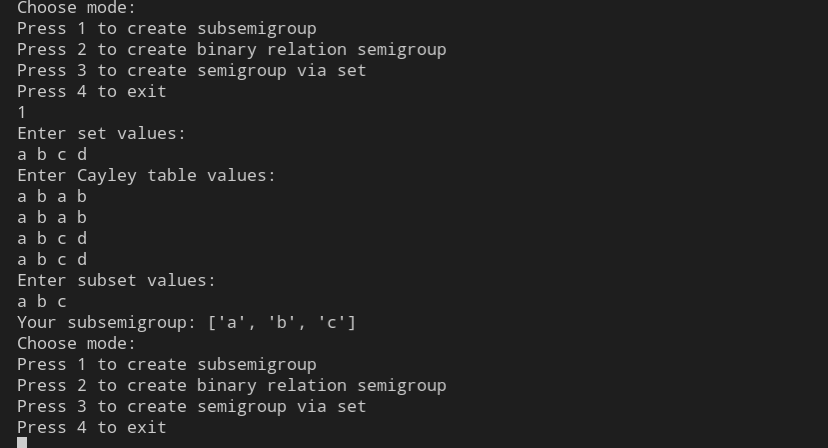
\includegraphics[width=0.8\textwidth]{photo/1.png}
        \caption{Тест алгоритма построения подполугруппы}
      \end{figure}

      На рисунках 2-4 изоражен результат работы алгоритма построения полугруппы с помощью булевых матриц.

      \begin{figure}[H]
        \centering
        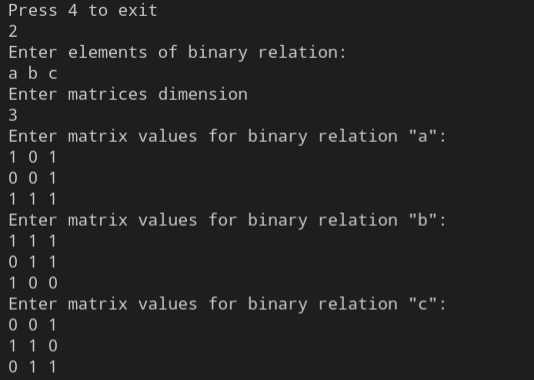
\includegraphics[width=0.8\textwidth]{photo/2.png}
        \caption{Тест алгоритма построения полугруппы с помощью булевых матриц}
      \end{figure}

      \begin{figure}[H]
        \centering
        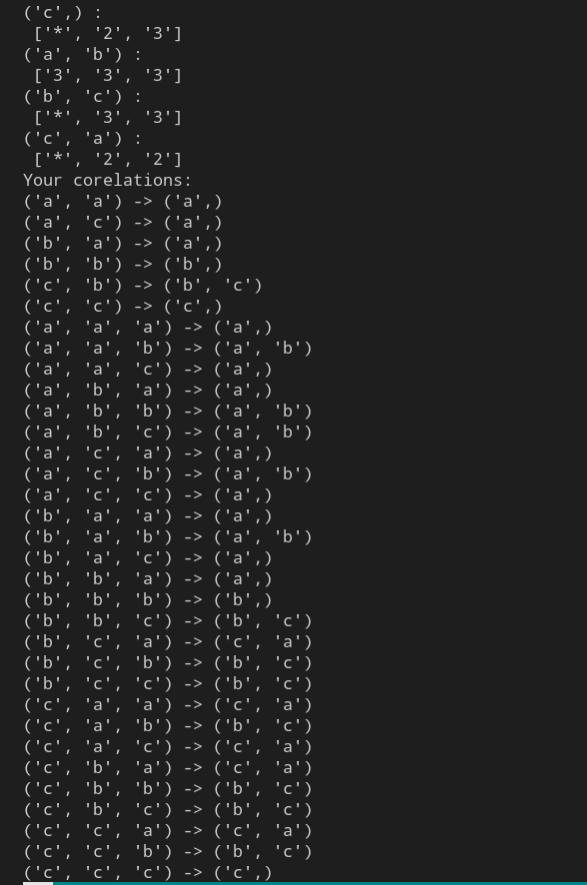
\includegraphics[width=0.8\textwidth]{photo/3.png}
        \caption{Вывод полугруппы, выраженной матрицами бинарных отношений}
      \end{figure}


      \begin{figure}[H]
        \centering
        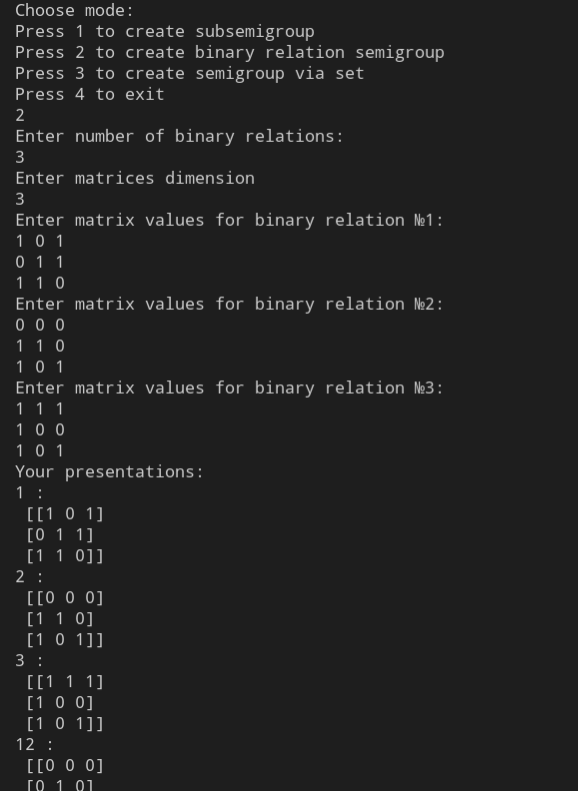
\includegraphics[width=0.5\textwidth]{photo/4.png}
        \caption{Вывод соотношений полугруппы (часть 1)}
      \end{figure}

      \begin{figure}[H]
        \centering
        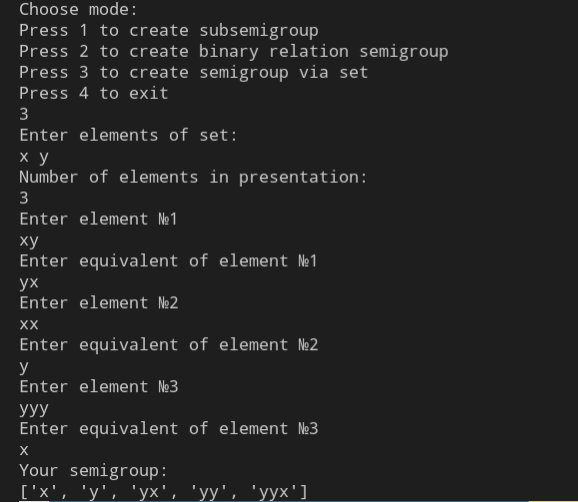
\includegraphics[width=0.8\textwidth]{photo/5.png}
        \caption{Вывод соотношений полугруппы (часть 2)}
      \end{figure}

      На рисунке 6 изоражен результат работы алгоритма построения полугруппы с помощью множества преобразований.

      \begin{figure}[H]
        \centering
        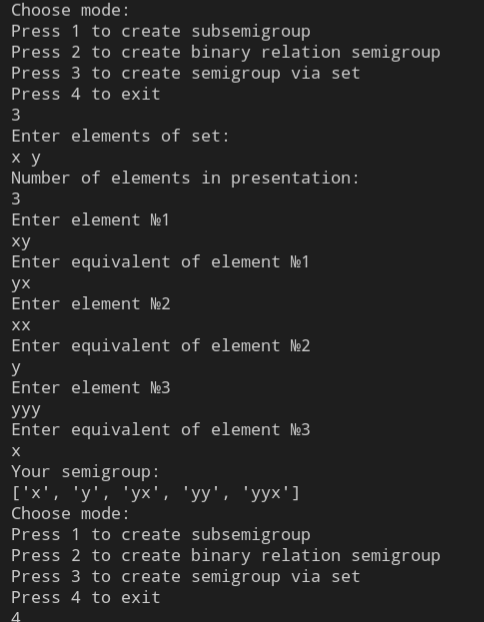
\includegraphics[width=0.7\textwidth]{photo/6.png}
        \caption{Тест алгоритма построения полугруппы с помощью множества преобразований}
      \end{figure}

    \subsection{Решение задач}
      \textbf{Задание 1.} Найдите полугруппу S = $\langle f, g \rangle$ преобразований множества $X = {1, 2, 3}$,
      порожденную следующими преобразованиями $f, g$ в симметрической полугруппе $T(X)$ преобразований множества $X$:
      \begin{center}
        $f = \begin{pmatrix}
          1 & 2 & 3 \\
          1 & 1 & 1
      \end{pmatrix}$,
        $g = \begin{pmatrix}
          1 & 2 & 3 \\
          2 & 3 & 2
        \end{pmatrix}$.
      \end{center}
    Известно, что множество преобразований $f, g$ порождает полугруппу S = $\langle f, g \rangle$ преоб-
    разований множества X, которая состоит из элементов $f, g, f^2 , fg, gf, g^2 , \dots $ и
    является подполугруппой конечной полугруппы $T(X)$.

    $f^2 = 
    \begin{pmatrix}
      1 & 2 & 3 \\
      1 & 1 & 1
    \end{pmatrix} \cdot
    \begin{pmatrix}
      1 & 2 & 3 \\
      1 & 1 & 1
    \end{pmatrix} = 
    \begin{tabular}{c c c c}
      & 1 & 2 & 3 \\
      f & $\downarrow$ & $\downarrow$ & $\downarrow$ \\
      & 1 & 1 & 1 \\
      f & $\downarrow$ & $\downarrow$ & $\downarrow$ \\
      & 1 & 1 & 1 \\
    \end{tabular} = 
    \begin{pmatrix}
      1 & 2 & 3 \\
      1 & 1 & 1
    \end{pmatrix}$

    $fg = 
    \begin{pmatrix}
      1 & 2 & 3 \\
      1 & 1 & 1
    \end{pmatrix} \cdot
    \begin{pmatrix}
      1 & 2 & 3 \\
      2 & 3 & 2
    \end{pmatrix} = 
    \begin{tabular}{c c c c}
      & 1 & 2 & 3 \\
      f & $\downarrow$ & $\downarrow$ & $\downarrow$ \\
      & 1 & 1 & 1 \\
      g & $\downarrow$ & $\downarrow$ & $\downarrow$ \\
      & 2 & 2 & 2 \\
    \end{tabular} = 
    \begin{pmatrix}
      1 & 2 & 3 \\
      2 & 2 & 2
    \end{pmatrix}$

    $gf = 
    \begin{pmatrix}
      1 & 2 & 3 \\
      2 & 3 & 2
    \end{pmatrix} \cdot
    \begin{pmatrix}
      1 & 2 & 3 \\
      1 & 1 & 1
    \end{pmatrix} = 
    \begin{tabular}{c c c c}
      & 1 & 2 & 3 \\
      g & $\downarrow$ & $\downarrow$ & $\downarrow$ \\
      & 2 & 3 & 2 \\
      f & $\downarrow$ & $\downarrow$ & $\downarrow$ \\
      & 1 & 1 & 1 \\
    \end{tabular} = 
    \begin{pmatrix}
      1 & 2 & 3 \\
      1 & 1 & 1
    \end{pmatrix}$

    $g^2 = 
    \begin{pmatrix}
      1 & 2 & 3 \\
      2 & 3 & 2
    \end{pmatrix} \cdot
    \begin{pmatrix}
      1 & 2 & 3 \\
      2 & 3 & 2
    \end{pmatrix} = 
    \begin{tabular}{c c c c}
      & 1 & 2 & 3 \\
      g & $\downarrow$ & $\downarrow$ & $\downarrow$ \\
      & 2 & 3 & 2 \\
      g & $\downarrow$ & $\downarrow$ & $\downarrow$ \\
      & 3 & 2 & 3 \\
    \end{tabular} = 
    \begin{pmatrix}
      1 & 2 & 3 \\
      3 & 2 & 3
    \end{pmatrix}$
    
    Таким образом получаем полугруппу: $S = \langle f, g, fg, g^2 , \dots \rangle$. Стоит отметить, что $gf \notin S$, так как
    $gf = f$. \\

    \textbf{Задание 2.}
    
    Найдите индекс и период следующих элементов $a$ полугруппы преобразований множества $X={1,2,3,4,5}$
    \begin{center}
      $a = 
    \begin{pmatrix}
      1 & 2 & 3 & 4 & 5 \\
      2 & 4 & 1 & 2 & 1
    \end{pmatrix}$
    \end{center}

    Посчитаем:
     
      $aa = 
      \begin{tabular}{c c c c c c}
        & 1 & 2 & 3 & 4 & 5\\
        a & $\downarrow$ & $\downarrow$ & $\downarrow$ & $\downarrow$ & $\downarrow$ \\
        & 2 & 4 & 1 & 2 & 1 \\
        a & $\downarrow$ & $\downarrow$ & $\downarrow$ & $\downarrow$ & $\downarrow$ \\
        & 4 & 2 & 2 & 4 & 2 \\
      \end{tabular} = 
      \begin{pmatrix}
        1 & 2 & 3 & 4 & 5 \\
        4 & 2 & 2 & 4 & 2
      \end{pmatrix}$ \\

      $aaa = 
      \begin{tabular}{c c c c c c}
        & 1 & 2 & 3 & 4 & 5\\
        a & $\downarrow$ & $\downarrow$ & $\downarrow$ & $\downarrow$ & $\downarrow$ \\
        & 2 & 4 & 1 & 2 & 1 \\
        a & $\downarrow$ & $\downarrow$ & $\downarrow$ & $\downarrow$ & $\downarrow$ \\
        & 4 & 2 & 2 & 4 & 2 \\
        a & $\downarrow$ & $\downarrow$ & $\downarrow$ & $\downarrow$ & $\downarrow$ \\
        & 2 & 4 & 4 & 2 & 4 \\
      \end{tabular} = 
      \begin{pmatrix}
        1 & 2 & 3 & 4 & 5 \\
        2 & 4 & 4 & 2 & 4
      \end{pmatrix}$ \\

      $aaaa = 
      \begin{tabular}{c c c c c c}
        & 1 & 2 & 3 & 4 & 5\\
        a & $\downarrow$ & $\downarrow$ & $\downarrow$ & $\downarrow$ & $\downarrow$ \\
        & 2 & 4 & 1 & 2 & 1 \\
        a & $\downarrow$ & $\downarrow$ & $\downarrow$ & $\downarrow$ & $\downarrow$ \\
        & 4 & 2 & 2 & 4 & 2 \\
        a & $\downarrow$ & $\downarrow$ & $\downarrow$ & $\downarrow$ & $\downarrow$ \\
        & 2 & 4 & 4 & 2 & 4 \\
        a & $\downarrow$ & $\downarrow$ & $\downarrow$ & $\downarrow$ & $\downarrow$ \\
        & 4 & 2 & 2 & 4 & 2 \\
      \end{tabular} = 
      \begin{pmatrix}
        1 & 2 & 3 & 4 & 5 \\
        4 & 2 & 2 & 4 & 2
      \end{pmatrix}$ \\

      Видно, что $aaaa \rightarrow aa$. Т.е. на 4 преобразовании наблюдается цикличность, тогда, если считать элементы полугруппы 
      $\langle a, aa, aaa, aaaa, ... \rangle$, начиная 
      с единицы, то каждый $2k$-й элемент будет иметь преобразование 
      $\begin{pmatrix}
        1 & 2 & 3 & 4 & 5 \\
        4 & 2 & 2 & 4 & 2
      \end{pmatrix}$, а каждый ($2k+1$)-й элемент равен --
      $\begin{pmatrix}
        1 & 2 & 3 & 4 & 5 \\
        2 & 4 & 4 & 2 & 4
      \end{pmatrix}$, где $k \in \mathbb{N}$. Получается, что период будет равен $2$.\\

    
    \textbf{Задание 3.}
    
    Найдите полугруппу $S$ по следующему ее копредставлению:
    \begin{center}

      $S = \langle x,y : xy = yx, x^2 = y, y^3 = x \rangle$
    \end{center}

    Выделим полную систему представителей классов конгруэнции $\epsilon$, которая определяется соотношениями данного
    копредставления. Для этого последовательно рассмотрим слова фиксированной длины и
    выделим те, которые не будут эквивалентны между собой относительно конгруэнции $\epsilon$.

    Рассмотрим слова длины 1: $x$, $y$ –- эти слова не эквивалентны между собой относительно конгруэнции $\epsilon$.

    Рассмотрим слова длины 2, которые получаются из слов
    длины 1 путем последовательного умножения их справа на буквы $x$ и $y$: $x^2 = y, xy, yx = xy, y^2$ -- из этих 
    слов только слова $xy$, $y^2$ не эквивалентны относительно конгруэнции $\epsilon$ другим ранее выделенным словам.

    Теперь рассмотрим слова длины $3$, которые получаются из выделенных слов длины $2$ путем последовательного
    умножения их справа на буквы $x$ и $y$: $xyx = y^2$, $xy^2$,  $y^2x = x^2y$, $y^3 = x$ –- из этих слов только
    слово $xy^2$ не эквивалентно относительно конгруэнции $\varepsilon$ другим ранее выделенным словам.

    Наконец рассмотрим слова длины $4$, которые получаются из выделенного слова длины $3$ путем последовательного
    умножения его справа на буквы $x$ и $y$: $xy^2x = x^2y^2 = y^3 = x$, $xy^3 = x^2 = y$ - все эти слова эквивалентны
    относительно конгруэнции $\varepsilon$ ранее выделенным словам.

        Значит, $S = \{x, y, xy, y^2, xy^2 \}$ "--- полная система представителей классов конгруэнции $\varepsilon$.
        Операция умножения $\cdot$ таких слов определяется с точностью до конгруэнции $\varepsilon$ по следующей таблице
        Кэли:

     \begin{table}[H]
          \centering
          \begin{tabular}{|c|c|c|c|c|c|}
          \hline
          $\cdot $ & $x$ & $y$  & $xy$  & $y^2$ & $xy^2$ \\ \hline
          $x$      & $x$ & $xy$ & $xy$  & $xy^2$ & $xy^2$ \\ \hline
          $y$      & $xy$ & $y^2$ & $xy^2$ & $y$ & $xy$ \\ \hline
          $xy$     & $xy$ & $xy^2$ & $xy^2$ & $xy$ & $xy$ \\ \hline
          $y^2$    & $xy^2$ & $y$ & $xy$ & $y^2$ & $xy^2$ \\ \hline
          $xy^2$   & $xy^2$ &  $xy$  &  $xy$ & $xy^2$ & $xy^2$ \\ \hline
          \end{tabular}
        \end{table}
    \conclusion
    
    В результате лабораторной работы были рассмотрены теоретические сведения о полугруппах, подполугруппах и
    порождающих множествах. Опираясь на изложенную
    выше теорию, были разработаны алгоритмы проверки свойств операций: ассоциативность, коммутативность, идемпотентность, обратимость,
    дистрибутивность, алгоритмы построения подполугруппы по таблице Кэли, построения
    полугруппы бинарных отношений по заданному порождающему множеству, построения полугруппы по порождающему множеству и
    определяющим соотношениям. Была произведена оценка сложности каждого из  построенных алгоритмов. Была реализована программа, написанная на языке Python
    с использованием библиотеки Numpy, Math, Itertools для работы с большими массивами данных.
    
\end{document}